\subsection{Обратная связь по выходу}
\selectlanguage{russian}

В предыдущих режимах входными блоками для функции шифрования были непосредственно блоки открытого текста. В режиме обратной связи по выходу (\langen{Output Feedback, OFB}, рис.~\ref{fig:OFB}) блоки открытого текста непосредственно на вход функции шифрования не поступают. Вместо этого функция шифрования генерирует псевдослучайный поток байтов (\emph{гамму}), который суммируется побитово по модулю $2$ с открытым текстом для получения шифртекста. Шифрование осуществляют по правилу:
\[ \begin{array}{l}
    K_0 = \textrm{IV}, \\
    K_j = E_K(K_{j-1}), ~ j = 1, 2, \dots, n, \\
    C_j = K_j \oplus M_j.
\end{array} \]

\begin{figure}[bt]
	\centering
	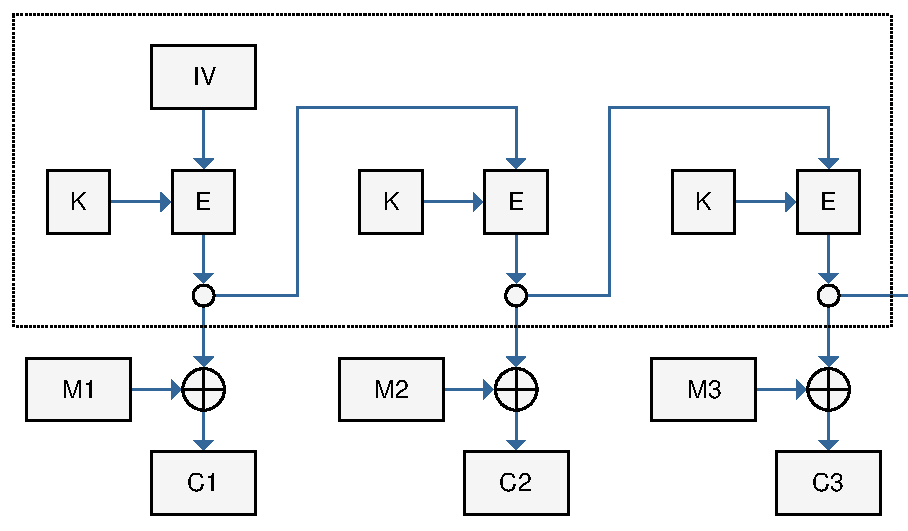
\includegraphics[width=1\textwidth]{pic/OFB}
	\caption{Режим обратной связи по выходу. Пунктирной рамкой выделена область формирования \emph{гаммы}, независящей от открытого текста.}
	\label{fig:OFB}
\end{figure}

Здесь текущий ключ $K_j$ есть результат шифрования предыдущего ключа $K_{j-1}$. Начальное значение $K_0$ известно криптографу и легальному пользователю. На приёмной стороне расшифрование выполняют по правилу:
\[ \begin{array}{l}
    K_0 = \textrm{IV}, \\
    K_j = E_K(K_{j-1}), ~ j = 1, 2, \dots, n, \\
    M_j = K_j \oplus C_j.
\end{array} \]

Как и в режиме CBC, вектор инициализации $\textrm{IV}$ может быть выбран случайно и передан вместе с шифрованным текстом, либо вычислен на основе одноразовых меток. Здесь особенно важна уникальность вектора инициализации.

Преимущества:
\begin{itemize}
	\item относительно простая реализация -- операции шифрования и расшифрования совпадают;
	\item нет необходимости дополнять открытый текст до размера, кратного размеру блоку шифрования;
	\item возможность частичной параллелизации шифрования (можно сгенерировать гамму до получения открытого текста);
	\item ошибка передачи одного бита приводит к ошибке в единственном бите открытого текста.
\end{itemize}

Недостатки:
\begin{itemize}
	\item непредсказуемый период (размер <<гаммы>>);
	\item не обеспечивает целостность.
\end{itemize}

Если рассматривать шифрование в режиме OFB как генератор псевдослучайной последовательности (<<гаммы>>), то очевидно, что максимальный период генератора равен $2^n$ блоков, где $n$ -- размер блока в битах. То есть максимальный период в битах равен $2^n \times n$. Однако нет никаких гарантий, что период будет максимален. Используя формулу из задачи о парадоксе дней рождения (см~\autoref{section:birthday-paradox}), находим, что математическое ожидание числа блоков, по достижению которого вероятность <<зациклиться>> более $1/2$, равно:

\[
b_{1/2} \geq \sqrt{2 \ln 2 \cdot N} \gtrapprox {1,18} \sqrt{N},
\]
где $N$ -- количество разных блоков. Так как $N = 2^n$, то

\[
b_{1/2} \gtrapprox \{1,18\} \sqrt{2^n} \gtrapprox {1,18} \cdot 2^{n/2}.
\]

Для шифров <<Кузнечик>> и AES $b_{1/2} \approx {1,18} \cdot 2^{64}$.

Данная оценка показывает математическое ожидание числа блоков. Но в реальности зацикливание может произойти даже на первом блоке, если в результате шифрования вектора инициализации $\textrm{IV}$ снова получится значение $\textrm{IV}$. Что фактически может привести к очень небезопасному шифрованию на гамме (<<гаммирование>>) с длиной периода всего в $n$ бит, где $n$ -- размер блока шифрования.

Хорошим размером гаммы считается такой, который больше размера шифруемого сообщения. То есть гамма не должна повторяться в рамках одной передачи. Теоретически можно ввести процесс отслеживания повтора гаммы (что на выходе функции шифрования получилось значение, равное $\textrm{IV}$) и перезапускать процесс передачи с другим значением вектора. Но это потребует усложнения режима шифрования, а также может привести к серьёзным проблемам, если при передаче нового значения $\textrm{IV}$ возникнет ошибка.

Данный режим (как и большая часть остальных рассмотренных режимов) обеспечивает только конфиденциальность\index{конфиденциальность} передачи данных, но не целостность\index{целостность}. В модели активного злоумышленника, если последний может предположить о содержимом любой части открытого текста, злоумышленник может поменять отдельные биты шифртекста, что приведёт к предсказуемым (с точки зрения криптоаналитика) изменениям в расшифрованном тексте.